\documentclass[tikz,border=0pt]{standalone}
\usepackage{sansmath}
\usepackage{siunitx}
\usetikzlibrary{calc}
\usepackage[T1]{fontenc}					%Schriften unterschiedlicher Kodierung
\usepackage[utf8]{inputenc}	

\begin{document}
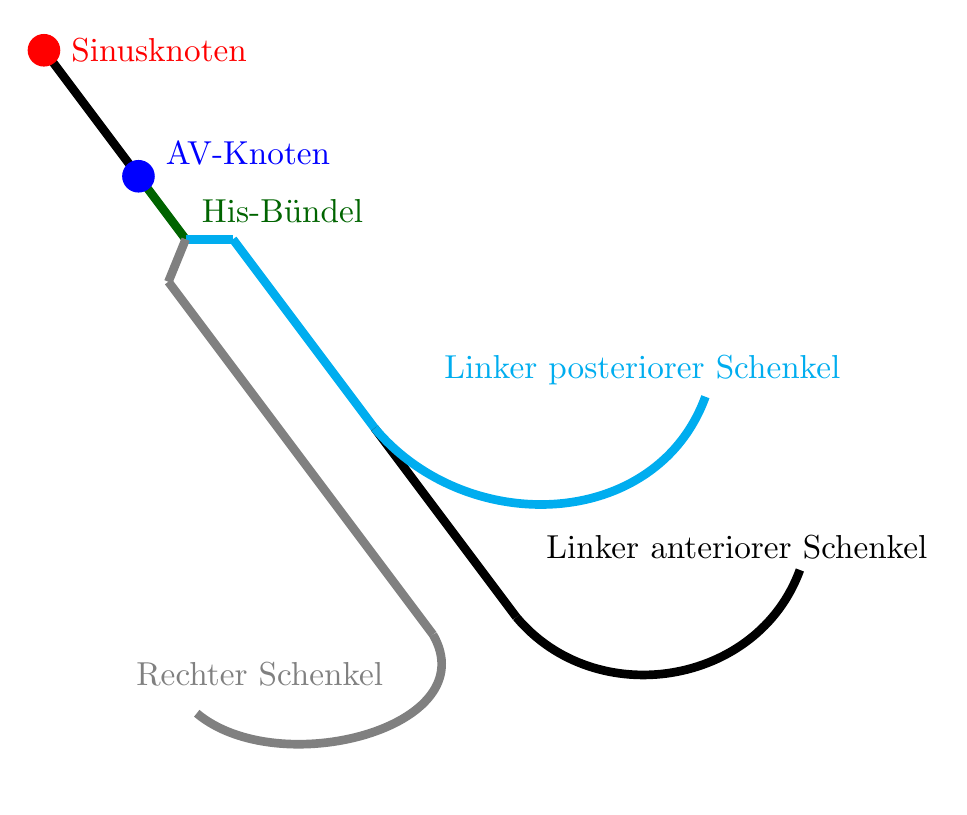
\begin{tikzpicture}


\def\gfxScale{2}
\def\lineWidth{1.1}
\def\textsize{1.2}
\def\nodedist{0.2}
\def\nodedistlong{0.8}
\definecolor{darkgreen}{RGB}{0,100,0}
\coordinate (center) at (0, 0);

\coordinate (sinus) at (0,0);
\coordinate (av) at ($(sinus) + \gfxScale*(0.6,-0.8)$);
\coordinate (his-ende) at ($(av) + \gfxScale*(0.3, -0.4)$);

\coordinate (linksschenkel-start) at ($(his-ende) + \gfxScale*(0.3, 0)$);
\coordinate (linksschenkel-kruemmung) at ($(linksschenkel-start) + \gfxScale*3*(0.6, -0.8)$);
\coordinate (linksschenkel-posterior-start) at ($0.5*(linksschenkel-start) + 0.5*(linksschenkel-kruemmung)$);
\coordinate (linksschenkel-posterior-ende) at ($(linksschenkel-start) + \gfxScale*(3, -1)$);
\coordinate (linksschenkel-kruemmung-ende) at ($(linksschenkel-kruemmung) + \gfxScale*(1.8, 0.3)$);

\coordinate (rechtsschenkel-start) at ($(his-ende) + \gfxScale*(-0.11, -0.27)$);
\coordinate (rechtsschenkel-kruemmung) at ($(rechtsschenkel-start) + \gfxScale*2.8*(0.6, -0.8)$);
\coordinate (rechtsschenkel-kruemmung-ende) at ($(rechtsschenkel-kruemmung) + \gfxScale*(-1.5, -0.5)$);


%DRAW

\draw[line width=\lineWidth mm] (sinus) -- (av);
\draw[fill, red] (sinus) circle (\gfxScale/10) ++ (\nodedist, 0) node[right, scale=\textsize] {Sinusknoten};
\draw[line width=\lineWidth mm, darkgreen] (av) -- (his-ende) ++ (0, 0) node[above right, scale=\textsize] {His-Bündel};
\draw[fill, blue] (av) circle (\gfxScale/10) ++ (\nodedist, 0) node[above right, scale=\textsize] {AV-Knoten};
\draw[line width=\lineWidth mm, cyan] (his-ende) -- (linksschenkel-start);
\draw[line width=\lineWidth mm, cyan] (linksschenkel-start) -- (linksschenkel-posterior-start);
\draw[line width=\lineWidth mm] (linksschenkel-posterior-start) -- (linksschenkel-kruemmung);

\path[line width=\lineWidth mm] (linksschenkel-kruemmung) edge[out=-50, in=-110, looseness=1.1] (linksschenkel-kruemmung-ende);
\draw (linksschenkel-kruemmung-ende) ++ (-\nodedistlong, 0) node[above, black, scale=\textsize] {Linker anteriorer Schenkel};
\path[line width=\lineWidth mm, cyan] (linksschenkel-posterior-start) edge[out=-50, in=-110, looseness=1.1] (linksschenkel-posterior-ende);
\draw (linksschenkel-posterior-ende) ++ (-\nodedistlong, 0) node[above, cyan, scale=\textsize] {Linker posteriorer Schenkel};

\draw[line width=\lineWidth mm, gray] (his-ende) -- (rechtsschenkel-start);
\draw[line width=\lineWidth mm, gray] (rechtsschenkel-start) -- (rechtsschenkel-kruemmung);
\path[line width=\lineWidth mm, gray] (rechtsschenkel-kruemmung) edge[out=-60, in=-40, looseness=1.1] (rechtsschenkel-kruemmung-ende);
\draw (rechtsschenkel-kruemmung-ende) ++ (\nodedistlong, \nodedist) node[above, gray, scale=\textsize] {Rechter Schenkel};


\end{tikzpicture}
\end{document}